\documentclass[5pt,letter]{article}
\usepackage{import}
\import{../../../sistema/}{rutas}
\usepackage[T1]{fontenc}
%\usepackage[letterpaper, headsep=60pt, headheight=2cm]{geometry}
\usepackage{verbatim}
\usepackage[utf8x]{inputenc}
\usepackage[table]{xcolor}
\usepackage{float}
\usepackage{import}
\usepackage{textcomp}
\usepackage{ifthen}
\usepackage[spanish,mexico-com]{babel}
\usepackage{pdflscape}
\usepackage{mathrsfs}
\usepackage{amsmath}
\usepackage{amssymb}
\usepackage{bbm}
\usepackage{tikz}
\usepackage{fp}
\usepackage[autolanguage]{numprint}
\usepackage{array}
\usetikzlibrary{shapes}
\usepackage{subfigure}
\usepackage{ucs}
\usepackage[utf8x]{inputenc}
\usepackage{fontenc}
\usepackage{graphicx}
\usepackage{anysize}
\usepackage{relsize}
\usepackage{booktabs}

\usepackage{fancyhdr}
\usepackage[all]{xy}
\setlength{\headheight}{13.1pt}
\makeatletter\renewcommand\theenumi{\@alph\c@enumi}\makeatother
\renewcommand\labelenumi{\theenumi)}
\usepackage{amsthm}
\usepackage{enumerate}

\usepackage[]{mdframed}

\usepackage{marvosym}
\usepackage{tikzsymbols}
\usepackage{imakeidx}%for indexes
%\usepackage{tocbibind}
\usepackage{background}
\usepackage{titlesec}
\usepackage{multirow}
\usepackage{etoolbox}
\usepackage{fmtcount}
\usepackage{datetime}
\usepackage[bookmarks=true]{hyperref}%must be at the end of preamble
\usepackage[toc,section=subsection, acronym, shortcuts]{glossaries}
\usepackage[open,openlevel=0]{bookmark}
\usepackage{lipsum}
\usepackage{multicol}
\usepackage{wrapfig}
\usepackage[titletoc]{appendix}
\usepackage{sectsty}

\usepackage{titlesec}
\usepackage{pdfpages}
%---------------Formato Numeros \numprint-------------
\npdecimalsign{.}
\nprounddigits{2}
\npthousandsep{,}

%-----------------Espacio en blanco--------------------
\newcommand{\espacio}[1]{\vspace{#1}\begin{center}\textit{[EL RESTO DE ESTA PÁGINA HA SIDO DEJADO EN BLANCO\\
DE FORMA INTENCIONAL]}\end{center}\newpage}
\newcommand{\inserta}{\colorbox{principal}{\textcolor{orange}{Insertar}}}
\usepackage{textcomp}
\decimalpoint
%------------Diseño de página --------------------------------
\usepackage[centering, letterpaper,margin=2cm,top=1cm, headsep=24pt, headheight=2cm,includehead, includefoot]{geometry}

%------------Colores----------------------

\definecolor{principal}{RGB}{0, 53, 73}
\definecolor{secundario}{RGB}{43, 82, 96}
\definecolor{terciario}{RGB}{43,82,96}

%--------------Hipervinculos en color, ligas-azul, archivos-magenta, url-azul----------------
\hypersetup{
    colorlinks=true,
    linkcolor=secundario,
    filecolor=magenta,      
    urlcolor=blue}

%-------------Encabezado---------------------
\pagestyle{fancy}
\fancyhf{}

\chead{
\includegraphics[width=8cm]{\rutaImagenes/logo_valuami_fondo_blanco}}

%--------------Pie de página------------------
\cfoot{\textbf{\textcolor{principal}{\footnotesize{VALUAMI\tiny\textregistered}}}\\ \scriptsize{\textit{Amargura 50, Interior 7 y 8, Antigua Granada Parques de la Herradura.\\ Huixquilucan, Estado de M\'exico. CP 52786.\\ Tel. 52 94 76 80 / 55 89 96 34\\ \url{www.ami-mexico.com/valuami}}}}

%------------Títulos de seccion y subseccion--------------



%\renewcommand \thechapter {\Roman{chapter}}
\renewcommand \thesection {\Roman{section}}
%\renewcommand \thesubsection {\thesection.\arabic{subsection}}
%\renewcommand \thesubsubsection {\thesection.\arabic{subsection}.\arabic{subsubsection}}

\titleformat{\section}[hang]{\color{gray}\huge\bfseries}{\thesection.}{1em}{} 

%\chapterfont{\color{principal}}
\sectionfont{\color{principal}}
%\subsectionfont{\color{secundario}}
%\subsubsectionfont{\color{terciario}}

%------------------Profundidad del índice---------------------------

\setcounter{tocdepth}{3}
\setcounter{secnumdepth}{3}




%------------------Marca de agua---------------

\backgroundsetup{angle=0, contents={
\includegraphics[width=8cm]{\rutaImagenes/logo_valuami_fondo_blanco}},opacity=.3, scale=1}



%----------------------------Generales----------------------------
\newcommand{\tipoAvaluo}{insertar}
\newcommand{\bienesValuados}{insertar}
\newcommand{\lugarInforme}{insertar}

%--------------------Fechas---------------------------
\newcommand{\diainforme}{insertar} %dia del informe
\newcommand{\mesinforme}{insertar} %mes del informe
\newcommand{\annoinforme}{insertar} %año del informe

\newcommand{\diavalores}{insertar} %dia de valores
\newcommand{\mesvalores}{insertar} %mes de valores
\newcommand{\annovalores}{insertar} %año de valores

\newcommand{\diainspeccion}{insertar} %dia de inspeccion
\newcommand{\mesinspeccion}{insertar} %mes de inspeccion
\newcommand{\annoinspeccion}{insertar} %año de inspeccion

\newcommand{\fechaInforme}{\diainforme{} de \monthname[\mesinforme] de \annoinforme}
\newcommand{\fechaValores}{\diavalores{} de \monthname[\mesvalores] de \annovalores}
\newcommand{\fechaValoresCorto}{\diavalores/\mesvalores/\annovalores}
\newcommand{\fechaInspeccion}{\diainspeccion{} de \monthname[\mesinspeccion] de \annoinspeccion}

%----------------------------Perito Valuador---------------------
\newcommand{\peritoValuador}{DiegoPerezcano}
\import{\rutaValuatex/documentos_modelo/peritos/peritos/}{\peritoValuador}

%------------------------Perito Auxiliar-------------------
\newcommand{\peritoAuxiliar}{DiegoPerezcano}
\ifthenelse{\equal{\peritoAuxiliar}{n/a}}{ }{\import{\rutaValuatex/documentos_modelo/peritos/auxiliares/}{\peritoAuxiliar}}

%--------------Datos del solicitante-------------
\newcommand{\empresaSolicitante}{insertar}
\newcommand{\empresaCorto}{insertar}
\newcommand{\rfcEmpresa}{insertar}
\newcommand{\personaSolicitante}{insertar}
\newcommand{\caracterSolicitante}{insertar}



\begin{document}
\begin{flushright}
\lugarCotizacion{} a \fechaCotizacion.\\
\textcolor{principal}{Asunto:} Propuesta de valuación\\
 \empresaSolicitante
\end{flushright}

\textcolor{principal}{\empresaSolicitante}\\

At'n.- \personaSolicitante.\\

Presente.\\

Agradecemos que haya considerado a nuestra firma, (en lo sucesivo ``Valuami''\textregistered{} y/o la ``Firma''), para la prestación de diversos servicios de valuación financiera (el “Proyecto”); por lo que hemos preparado la siguiente propuesta:

\begin{center}
\section{PROPUESTA DE VALUACIÓN DE \empresaSolicitante}
\end{center}

\textcolor{principal}{SERVICIOS.-} Elaboración de un Dictamen de VALUACIÓN independiente respecto del Valor del \textbf{negocio en marcha} y \textbf{capital accionario} del negocio \textcolor{principal}{\empresaSolicitante}\\

 
 \begin{itemize}
 \item \underline{Propósito:} Estimar el valor razonable del negocio en marcha (\textit{Firm Value}) y de su capital accionario (\textit{Equity Value}), con fecha de valores al 31 de Diciembre de 2023 (cierre del último ejercicio).
 
\item \underline{Uso:} Se utilizará para efectos informativos.
 
 \end{itemize}
 
 \begin{center}
 \section{ENFOQUES DE VALUACIÓN A SER APLICADOS.}
 \end{center}
 
Los enfoques de valuación más utilizados para valuar un negocio en marcha, son los
 siguientes:
 
 \begin{figure}[H]
 \centering
 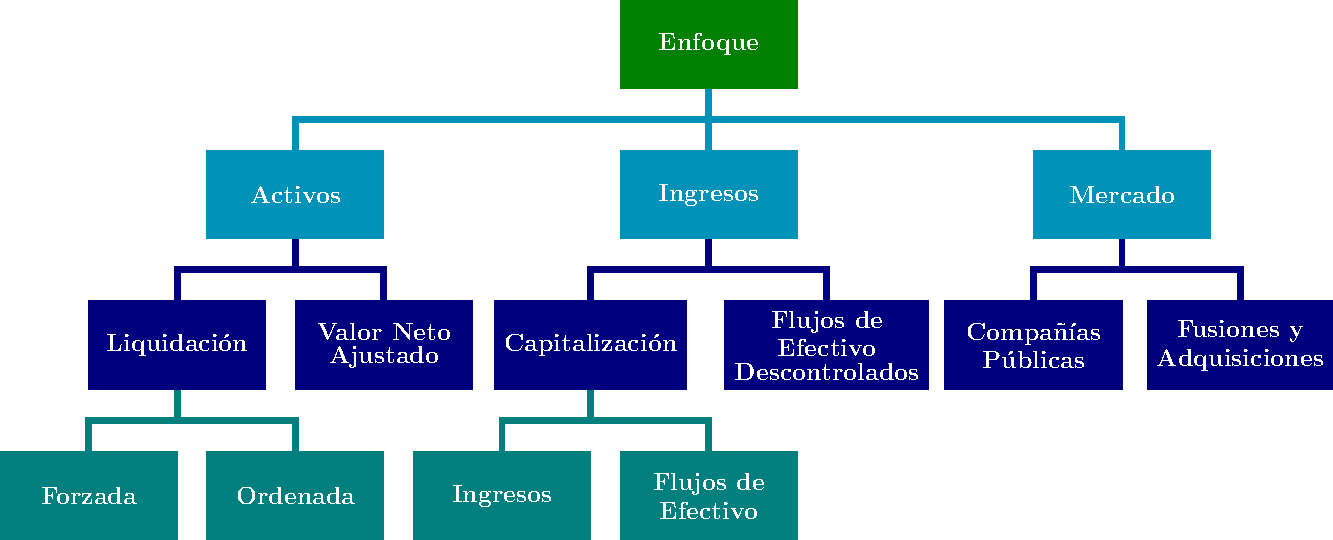
\includegraphics[width=.8\textwidth]{\rutaImagenes/enfoques_mas_utilizados}
 \end{figure}
 
 \begin{itemize}
 
\item  Enfoque de Activos. Este enfoque considera que para determinar el valor de un negocio en
 marcha, se requiere determinar el valor de reposición de las inversiones asociadas a su
 aprovechamiento económico.
 

\item Enfoque de Ingresos. Este enfoque asigna el valor de un negocio en marcha a su capacidad
 de generar flujos de efectivo y de obtener un retorno razonable sobre su inversión.
 
\item  Enfoque de mercado. El enfoque empírico consiste en determinar el valor de un negocio en
marcha con base en el valor de razones o relaciones derivadas del análisis de los precios de
operaciones intangibles o de transacciones de compañías públicas, aplicables al activo
analizado. Tanto la información de fusiones y adquisiciones, así como la actividad de
compraventa de títulos accionarios sirven para obtener medidas aplicables.

\end{itemize}

 \begin{center}
 \section{METODOLOGÍA DE VALUACIÓN DE NEGOCIOS.}
 \end{center}
 
 Se utilizarán para dicha valuación alguno(s) de los siguientes métodos financieros, entre
otros:\\	
 
\begin{itemize}
\item Método de Flujos de Efectivo Descontados (\textit{DCF Valuation})
\item Método de Valuación Relativa (\textit{PEERS Valuation}).
\item Método EVA (\textit{Valor Agregado Estimado})
\end{itemize}

 \begin{center}
 \section{CONDICIONES DEL SERVICIO.}
 \end{center}
 
\textcolor{principal}{Tarifas y facturación:} En relación con nuestro sistema de facturación, al igual que la mayor parte de los despachos de consultoría financiera, nuestros honorarios se facturan con base en el tiempo efectivamente dedicado a cada asunto, y con tarifas que varían dependiendo del
nivel y experiencia del CONSULTOR involucrado; a las cuales se deberá agregar el Impuesto
al Valor Agregado que corresponda.\\


\textcolor{principal}{COTIZACIÓN:} De acuerdo con nuestra experiencia en estas valuaciones, el importe de honorarios por los servicios en esta Propuesta corresponderán a \textcolor{principal}{MXN \honorarios{}  + IVA}(\honorariosLetra{} pesos 00/100 moneda nacional, más el impuesto al valor agregado aplicable):

 \begin{figure}[H]
 \centering
 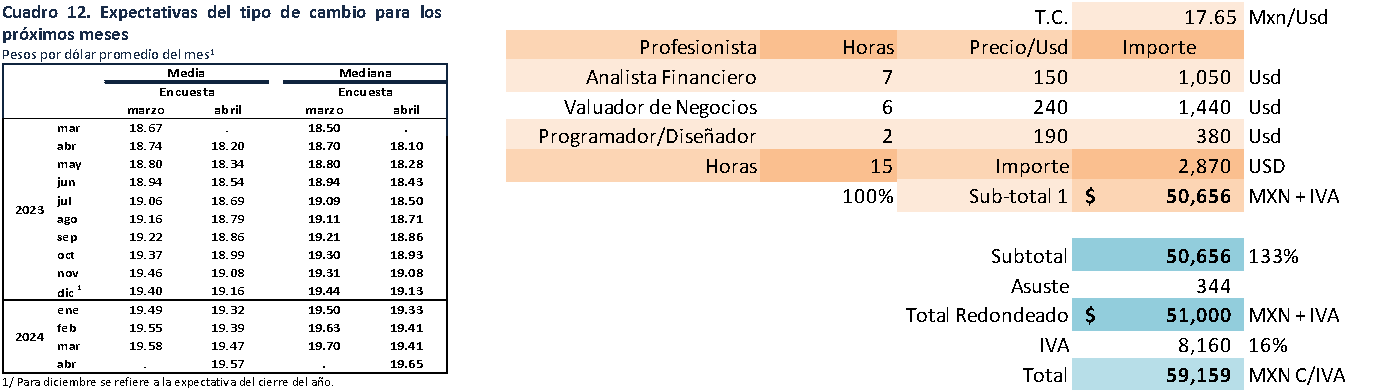
\includegraphics[width=.9\textwidth]{cotizacion_1}
 \end{figure}



\begin{center}
\section{ALCANCES DEL SERVICIO:}
\end{center}

Para lograr la realización del proyecto, los honorarios propuestos por la FIRMA se detallan según se describe:\\
 
 \begin{enumerate}[a)]
 \item Respecto de los servicios que se detallan, se requerirá un anticipo de \$\anticipo{} MXN
 + IVA.
 
 \item Se requerirá un monto restante contra entrega del avalúo que corresponda, por un
 importe de \$\liquidacion{} MXN + IVA.
 
 \end{enumerate}
 
 Es importante mencionar que los honorarios únicamente cubren nuestros servicios, por lo que
de ninguna forma deberá entenderse que los mismos incluyen de manera enunciativa y no
limitativa honorarios por otros servicios financieros y/o cualquier otro concepto no incluido
en la presente propuesta de servicios.\\
 
 \begin{itemize}
\item Tiempo de ejecución: 15 días hábiles, a partir de contar con la información completa.\\
\item  La presente cotización tiene vigencia de 30 días.\\
\item  Los honorarios del perito valuador no están condicionados a la obtención de un valor
determinado.\\
\end{itemize}
 
Datos bancarios: Asesoría Mercantil Integral, S.C.- Clabe BBVA: 012180001923895173.
Total con impuestos: \$\totalMasIva{} pesos.
 
\begin{center}
\section{REQUERIMIENTOS DE INFORMACIÓN:}
\end{center}
 
 A continuación enlistamos el requerimiento de información para comenzar el análisis de valuación. No es necesario agotar todo el listado, salvo la información financiera indispensable (estados financieros) y jurídica. Todo lo demás es optativo y nos ayuda a realizar un mejor trabajo. Se sugiere que la transmisión de la información fuese a través de un Data Room Digital con el objetivo de facilitar la transmisión de la misma.\\
 
 \begin{enumerate}[a)]
 \item Información financiera de la Sociedad que factura los ingresos de la sociedad:
 \begin{itemize}
\item Estados financieros históricos de 5 años a la fecha (auditados o en su caso internos): i) Estado de resultados, ii) Estado de situación financiera, iii) Estado de flujos de efectivo, iv) Estados de variaciones al capital contable, v) Notas a los estados financieros.
\item Estados financieros internos al último trimestre disponible: i) Estado de resultados, ii) Estado de situación financiera.
\item Relación analítica de Costos y Gastos de administración.
\item Relación analítica de propiedades, planta y equipo.
\item Listado de créditos bancarios y no bancarios, con fecha, costo y vigencia.
\item Proyección de ingresos para los próximos 5 años realizada por la empresa (en
caso de contar con esa información).
\item Declaración anual de impuesto del último año (para revisar los atributos fiscales
del negocio).
\end{itemize}
\item  Información de negocios de la sociedad:
\begin{itemize}
\item Presentación corporativa (Brochure de negocios).
\item Unidades de negocio y sus marcas registradas (con su título de registro).
\item Listado de Principales clientes, actuales y potenciales.
\item Organigrama.
\item Ejecutivos clave.
\end{itemize}
\item Información Jurídica de la sociedad:
\begin{itemize}
\item Acta constitutiva de la sociedad.
\item Protocolizaciones de actas de asamblea relevantes.
\item Cualquier otra certificación o contrato que sea relevante para el estudio (Permisos
Sanitarios, Certificación de Normas oficiales mexicanas (NOM), Título(s) de concesión, entre otros).
\end{itemize}
\end{enumerate}

  \begin{center}
 \section{OTROS:}
 \end{center}
 
 El propósito de la presente es definir únicamente los términos más importantes bajo los cuales la Firma prestaría sus servicios a usted, por lo que si tuvieran cualquier duda les pedimos nos lo haga saber a la brevedad para abundar más en el tema, incluyendo tópicos como conflicto de interés, código de ética y conducta, resguardo y entrega de documentos, áreas y perfiles de práctica, operaciones relevantes de la Firma, etc.\\
 
En caso de que estuviera de acuerdo con la presente propuesta, agradeceremos se sirva firmar de conformidad en el espacio que se indica al final de esta y hacernos llegar una copia por este medio.\\
 
 La firma de esta propuesta será una confirmación de su autorización para que la FIRMA y/o VALUAMI los asesoren en los asuntos que se describen en la presente comunicación, así como en aquéllos otros que nos indiquen y refieran eventualmente.\\
 
 La interpretación y cumplimiento de la presente estará sujeta a las leyes de la Ciudad de México y a los tribunales competentes con residencia en dicha capital.\\
 
 Agradecemos nuevamente su confianza y esperamos que encuentren la presente satisfactoria a efecto de poder asesorarlos en relación con el proyecto.\\		
 
 Atentamente,\\
 
\begin{minipage}{.7\textwidth}
 \textcolor{principal}{Mtro. Diego M. Perezcano}\\
 Perito valuador de Negocios en Marcha, Cédula SEP 10548258\\
 Corredor Público Número 2 de la Plaza del Estado de México\\
 \url{dperezcano@ami-mexico.com}
 \end{minipage}
 
 
\includegraphics[width=2cm]{\rutaImagenes/nyulogo}\\
 
 \begin{flushright}
\textcolor{principal}{Aceptado de conformidad en todos sus términos:}\\[10pt]

\rule{5cm}{1pt}\\
\textcolor{principal}{Por: \personaSolicitante}\\
\textcolor{principal}{Cargo: \caracterSolicitante}

 \end{flushright}
 
 
 
 

\end{document}